Recovery and downblending of \gls{HEU} to produce \gls{HALEU} means that 
the fuel contains impurities present in the original
\gls{HEU}. Known impurities in potential \gls{HEU}
supplies to create \gls{HALEU} include $^{232}$U and $^{236}$U
\cite{vaden_isotopic_2018,nelson_foreign_2010},  
which are parasitic neutron absorbers and have the potential to affect 
reactor physics and reactor operation. To investigate the magnitude of this 
effect, this chapter presents models of the use of 
impure \gls{HALEU} fuel in a reactor and compares it to the use of pure 
\gls{HALEU} (comprised exclusively of $^{235}$U and $^{238}$U). This analysis 
helps in understanding the impacts of the impurities on the performance of the reactor.
While the other chapters explore how the reactors affect the fuel cycle this 
chapter of work explores how the fuel affects the reactors.  We determined 
the downblended \gls{HALEU} compositions based on what is publicly 
available. 




\textbf{ASTM has standards on UOX/MOX purity -- ASTM C776-06, C753 (2004), C757 (2006a)}

\section{Methodology}\label{sec:neutronics-methods}
For this work we considered the two \gls{HALEU}-fueled reactors modeled 
in the transition scenarios described in Chapter \ref{ch:fc_methods}. 
Full core models of Xe-100-like and 
\gls{MMR}-like reactors were created in Serpent 
\cite{leppanen_serpent_2014} to model the neutronics and depletion of fuel 
in each reactor design. Each model was run using the ENDF VII.1 
cross section library
\cite{chadwick_endfb-vii1_2011}. The core geometries used are not 
the exact geometries designed by X-energy and \gls{USNC}, respectively, but 
are replications based on publicly-available information 
\cite{mulder_overview_2021,nuscale_chapter_2020,reyes_nuscale_2021,reyes_correction_2022}. 

\subsection{Xe-100-like model}
The Xe-100 is a \acrfull{TRISO}-fueled pebble-bed \gls{HTGR} with a power 
output of 80 MWe \cite{mulder_overview_2021}. To model this reactor
we used the Sanagmon200 model from \cite{richter_isotopic_2022}, shown in 
Figure \ref{fig:xe100_core}, to serve as an Xe-100-like 
core model. The model itself can be found on GitHub \cite{richter_zoerichterphlox_2022}.
The Sangamon200 model is a \acrfull{TRISO}-fueled, pebble-bed, \gls{HTGR}-style 
reactor core model 
initially created to characterize the isotopic compositions and 
reactor physics of a 200 MW pebble-bed \gls{HTGR}. While this reactor model 
is very similar to current published data for the X-energy Xe-100
\cite{mulder_overview_2021}, there are some notable differences that affect 
the reactor physics. The first difference is that the \gls{TRISO} particles 
in the Sangamon200 are modeled as a blended mix of the \gls{TRISO} 
materials, not the explicit layers. Using a homogenized \gls{TRISO} particle 
decreases the \keff of the core by 4.45\%, but it does not reduce the 
thermal and fast neutron fluxes across the reactor outside of error 
\cite{richter_isotopic_2022}. Despite 
the effect on \keff of this modeling decision, we continued to use the 
homogenized model of the \gls{TRISO} pebbles to be consistent with the 
published results of the Sanagamon200 \cite{richter_isotopic_2022} and 
to be conscious of computational expense. 

\begin{figure}[ht]
    \centering 
    \begin{subfigure}{0.45\textwidth}
        \centering 
        \includegraphics[scale=0.03]{htgr-mr-full-core.inp_geom1.png}
        \caption{Radial view of Xe-100-like core model.}
        \label{fig:xe100_core_radial}        
    \end{subfigure}
    \hfill
    \begin{subfigure}{0.45\textwidth}
        \centering 
        
\includegraphics[scale=0.12]{htgr-mr-full-core.inp_geom3.png}
        \caption{Axial view of Xe-100-like core model.}
        \label{fig:xe100_core_axial}        
    \end{subfigure}
    \caption{Xe-100-like core model made in serpent.}
    \label{fig:xe100_core}
\end{figure}

The second 
notable difference is the reactor vessel shape. The Sanagmon200 is a simple 
cylinder, while the Xe-100 is a cylinder with a cone at the bottom to funnel 
the pebbles to a single point as they come out of the core. However, 
this is a lss neutronically important region of the core, so the geometry 
difference between the two cores should produce a negligible effect on the results of the 
core as a whole.

In the Xe-100 reactor, each pebble moves down the core while it burns. Each 
time that a pebbles travels from the top of the core to the bottom is a single 
pass. Once a pebble reaches the bottom of the core, it is removed, inspected for 
the burnup level, and placed back in the core for another pass if the pebble has 
not reached the target burnup. Therefore, each pebble is expected to 
go through multiple passes in the core, an average 
of six passes per pebble. To account for the different burnup of 
the pebbles in an equilibrium core, 
six different pebble isotopic compositions were used to approximate the pebble
variance in burnup in the core. These isotopic compositions represent burnup from 
integer numbers of passes through the core.
To determine the isotopic composition of the 
pebbles after each pass we performed the methodology 
Richter developed for their modeling of the Sangamon200 \cite{richter_isotopic_2022}. 
We performed depletion on the single pebble model with each layer of the 
\gls{TRISO} kernel modeled
created by Richter \cite{richter_zoerichterphlox_2022} with depletion steps 
corresponding to integer numbers of passes. Then we 
applied the composition corresponding to the burnup step of each pass 
to 1/7th of the pebbles of the core. The pebbles with different burnups 
were evenly mixed throughout the core, mimicking spread of 
differently burned pebbles throughout a core in the equilibrium state 
of the reactor. Each pebble at the same burnup level has the same 
composition in this model.   

The Sangamon200 is modeled an an isothermal state at 800 K \cite{richter_isotopic_2022}.
We ran this model with 100,000 particles per cycle, 50 inactive cycles, 
and 200 active cycles. We did not perform depletion on the Sangamon200 model 
because our model 
does not capture the continuous refueling scheme used by the Xe-100 or 
any pebble movement. Performing depletion without modeling pebble movement 
would create non-physical differences from the equilibrium condition of 
this reactor model. Therefore, we did not model further depletion of the 
pebbles when comparing the different fuel compositions.

\subsection{MMR-like model}
The \gls{USNC} \gls{MMR} is an  \gls{HTGR} that uses 
\gls{TRISO} fuel in \acrfull{FCM} pellets inside graphite blocks 
to produce 5 MWe \cite{noauthor_usnc_2021}.
We created an \gls{MMR}-like model primarily based on information in 
\cite{hawari_development_2018}, and supplemented or modified based on 
information published by \gls{USNC} \cite{noauthor_usnc_2021}. 
Information about the \gls{TRISO} 
particle and \gls{FCM} pellets was found in \cite{noauthor_usnc_2021}
and information about the graphite block dimensions and configuration 
was found via visual inspection of figures in \cite{venneri_micro_2019}. 
The final core configuration 
is different than what is modeled by Hawari and Venneir \cite{hawari_development_2018} 
because their model is only meant to operate 
for 10 years, while the \gls{MMR} is meant to operate for 20 years 
\cite{noauthor_usnc_2021}. We 
selected this core configuration after modeling some of the other core 
configurations found in literature \cite{mitchell_usnc_2020,hawari_development_2018}
and determining that the core configuration shown in Figure \ref{fig:mmr_core} 
can operate the longest before going subcritical and 
achieve a burnup close to the reported 82.6 MWd/kgU reported by 
\gls{USNC} \cite{noauthor_usnc_2021}. 

Figure \ref{fig:mmr_core} shows a radial and axial slice of the 
\gls{MMR} model. The fuel channels have a radius of 1.15 cm, the same
size as the \gls{FCM} pellets based on no other available information, 
the coolant channels have a radius of 
3 cm, arbitrarily chosen because no specific information was found, 
and the control rod channels have a radius of 6 cm, obtained from 
\cite{hawari_development_2018}. These dimensions affect the graphite volume 
of the core, and thus affect the fuel to moderator ratio of the core. 
The \gls{TRISO} particles are modeled with a 40\% packing fraction in 
the \gls{FCM} particles based on information in .
Control rods and burnable poisons are not included in this model, or 
the Sangamon200 model, so the control rod locations are modeled as 
filled with helium. There are five layers of the graphite fuel blocks 
stacked to form the entire core, to approximate the number of 
fuel blocks described in \cite{noauthor_usnc_2021}. The entire core 
is assumed to be in an isothermal state at 800 K. There is a 20 cm 
thick graphite reflector above and below the stacks of graphite, 
and a 10 cm thick beryllium-oxide reflector on the outside of the 
graphite blocks of the core, illustrated by the green material in 
Figure \ref{fig:mmr_core}. Both axial graphite and radial 
beryllium reflectors are specified 
in \cite{hawari_development_2018}, with the thickness of the 
beryllium-oxide reflector given. However, the thickness of the graphite 
reflectors above and below the core was not specified, so we selected 
20 cm to provide 3-5 mean free paths of material. 
The input files for this model can be found at \textbf{create zenodo 
object}.

\begin{figure}
        \begin{subfigure}{0.48\textwidth}
                \centering
                
\includegraphics[scale=0.1]{bachmann-mmr_geom1.png}
                \caption{Radial view of the USNC MMR-like model.}
                \label{fig:mmr_radial}
        \end{subfigure}
        \hfill 
        \begin{subfigure}{0.48\textwidth}
                \centering
                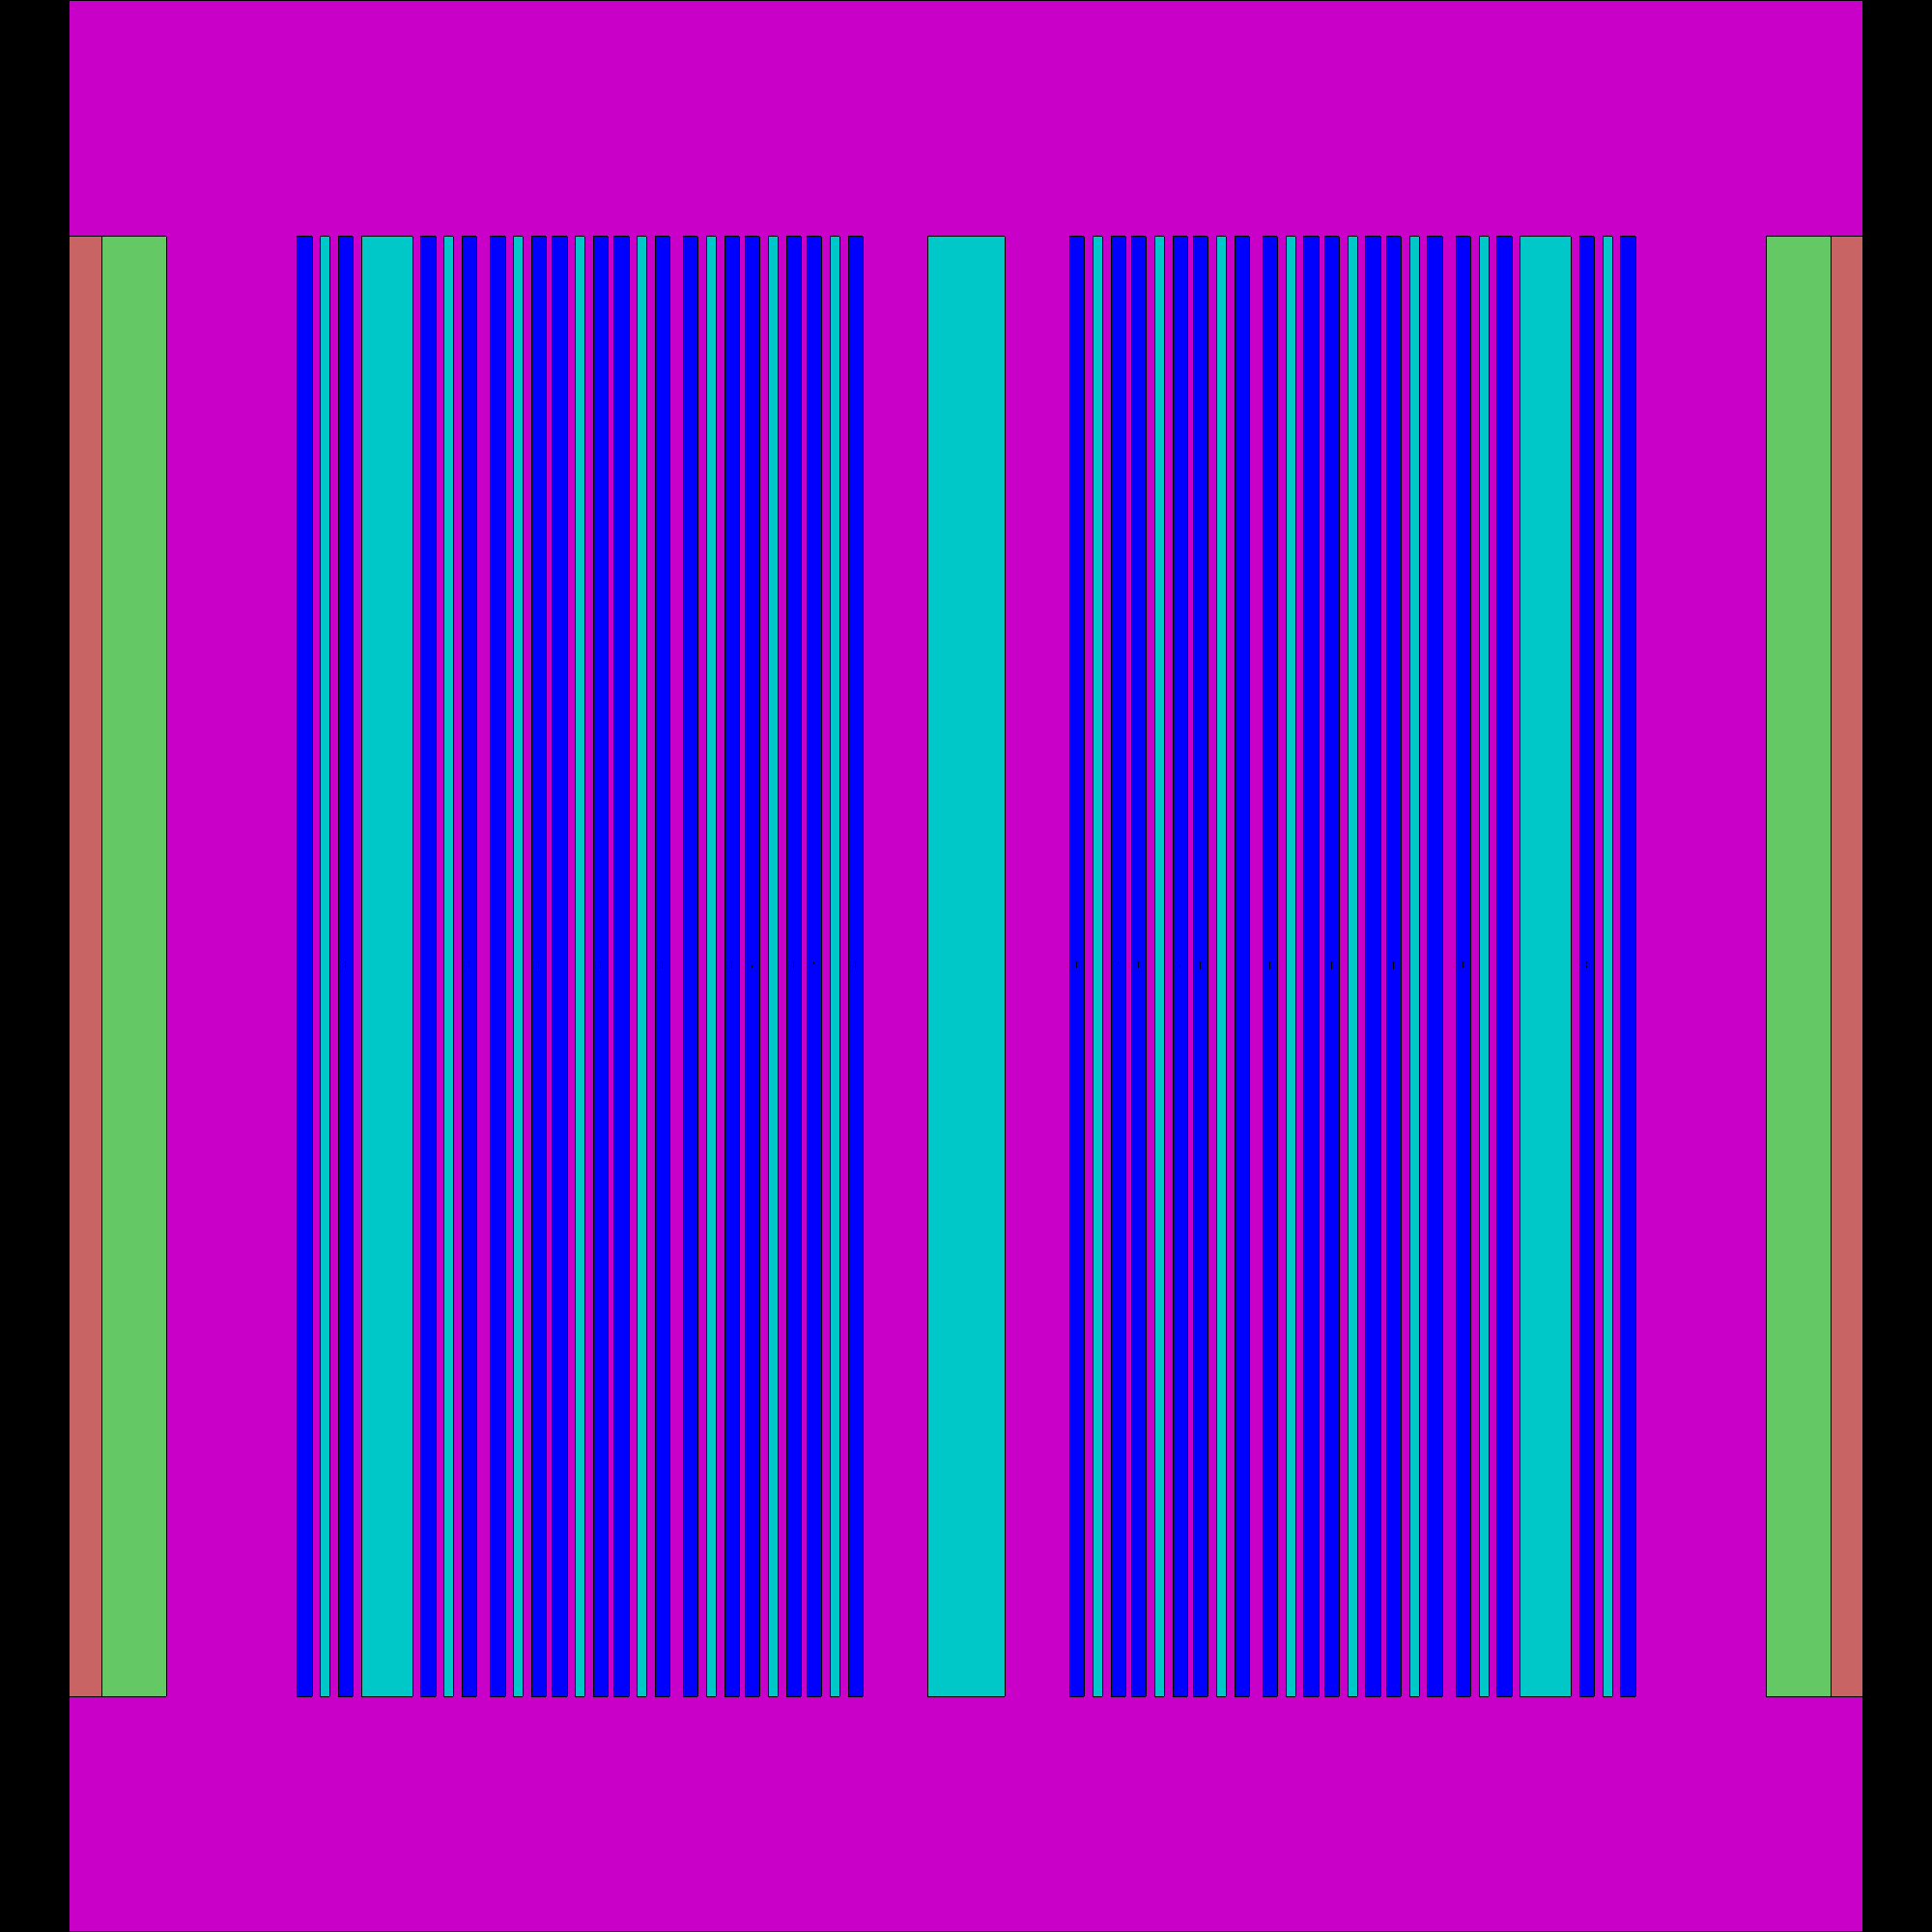
\includegraphics[scale=0.1]{bachmann-mmr_geom3.png}
                \caption{Axial view of the USNC MMR-like model.}
                \label{fig:mmr_axial}
        \end{subfigure}
        \caption{Geometry of USNC MMR-like core model in Serpent. The 
        light blue represents channels helium, dark blue are fuel 
        channels with \gls{FCM} pellets, and the bright pink is graphite in the core.}
        \label{fig:mmr_core}
\end{figure}

For the \gls{MMR}-like model we modeled depletion of the core across the 
expected 20 year lifetime of the \gls{MMR}, because the core is not 
meant to undergo refueling during those 20 years and the lack of 
fuel movement is in a state model aligned with the operational core. 
Depletion is modeled using 
burnup steps of 2 years. Each burnup step was run using 140 active cycles, 75 inactive 
cycles, and 65,000 particles per cycle. 

\subsection{Temperature variations and feedbacks}
For both reactor models, we varied the fuel, coolant, and moderator temperatures 
between 700, 750, 800, 850, and 900 K to calculate the fuel, coolant, 
moderator, and total temperature feedback coefficients. We assumed a linear 
relationship between 
\keff and temperature to calculate the feedback coefficients. When varying the 
temperatures of each component, we also varied the corresponding material 
density. We calculated the 
density of the UO$_2$ by using the empirical relationship between density and 
temperature defined in \cite{fink_thermophysical_2000}. The calculated 
densities were assumed to hold true for the Sangamon200. 
We calculated the 
graphite density by linearly extrapolating from the data available in 
\cite{mceligot_thermal_nodate}. We calculated the density of the helium 
by interpolating on the data available in \cite{petersen_properties_nodate}, 
assuming the 3 MPa coolant pressure in the \gls{MMR}-like model as defined 
by \cite{noauthor_usnc_2021} and the 6 MPa inlet pressure defined in 
\cite{mulder_overview_2021}. 

\subsection{Fuel compositions}
We used three different \gls{HALEU} compositions for this work: pure 
\gls{HALEU}, and \gls{HALEU} derived from \gls{EBR} and Y-12 \gls{HEU} 
stockpiles. The pure fuel composition assumes that all uranium present is 
either $^{235}$U or $^{238}$U, and at the correct enrichment level for each 
reactor. The \gls{EBR} 
composition is based on the estimated uranium isotopic composition from 
downblending spent fuel from \gls{EBR}, published by \gls{INL} 
\cite{vaden_isotopic_2018}. The Y-12 composition is based on the 
estimated uranium isotopic composition from downblending \gls{HEU} 
stockpiles at the Y-12 National Security Complex \cite{nelson_foreign_2010}.
The published isotopics for the \gls{EBR} and Y-12 fuel assume an enrichment 
of 19.75\%, but only the \gls{MMR} requires this level of enrichment. 
Therefore, for the fuel in the \gls{MMR}, the uranium isotopic ratios 
published are applied as part of the fuel composition. For the fuel in the 
Xe-100, the isotopic fractions had to be adjusted slightly to match the 
needed enrichment level. The $^{235}$U fraction was set to match the 
enrichment level required, the non-$^{238}$U isotopes were kept in the 
same ratio defined in the publications, and the $^{238}$U was defined to fill 
the remainder of the fuel. Therefore, all three fuel compositions for each 
reactor have the same $^{235}$U weight fractions, non-$^{238}$U weight
fractions that match the published values, and vary in the $^{238}$U 
weight fraction. 

\section{Results}
The points of comparison for this work include:
\begin{itemize} 
        \item \keff 
        \item \betaEff
        \item Neutron flux
        \item Reactivity temperature feedback coefficients
\end{itemize}

For the Sangamon200, these metrics are only compared for the initial 
state of the reactor. For the \gls{MMR}-like reactor these metrics 
are compared at \gls{BOL}, mid-cycle, and \gls{EOL}. Each metric provides a 
measurement of the performance of 
the reactor, such as the materials degradation rate, amount of burnable 
poisons required, control rod worth, and the cycle time. Investigating 
each of these results helps to determine if the impurities potentially 
present in \gls{HALEU} will prevent any of the design criteria of the 
reactors from being met. Results from the simulations are analyzed using 
the serpetnTools python package \cite{johnson_serpenttools_2020}. 

\subsection{Xe-100 reactor}

\subsubsection{\keff}
Table \ref{tab:xe100_keff} reports the \keff value when using each fuel 
composition. The impure fuels result in a \keff 1353-1423 pcm 
greater than the \keff from the pure fuel. All three fuel compositions 
result in a slightly super-critical \keff. The difference in the \keff 
values is more than the error on the values, which means that the 
different fuel compositions result in statistically different \keff 
values for this reactor design. 

\begin{table}[ht]
        \centering 
        \caption{\keff values for the Xe-100-like reactor model for 
        each fuel composition.}
        \label{tab:xe100_keff}
        \begin{tabular}{c c}
                \hline
                Fuel composition & \keff \\
                \hline 
                Pure & 1.06663 $\pm$ 0.00016\\
                \gls{EBR} & 1.08086 $\pm$ 0.00016\\
                Y-12 & 1.08016 $\pm$ 0.00014\\
                \hline                
        \end{tabular}
\end{table}

The uranium isotopes mostly 
present in 
each of the fuel compositions (weight fraction of at least 1$\times 10^{-3}$)
are $^{234}$U, $^{235}$U, $^{236}$U, and $^{238}$U. The $^{235}$U weight 
fraction is the same in each fuel composition, so the impurities are 
displacing the $^{238}$U in the fuel. $^{234}$U and $^{236}$U have larger 
total fission cross sections than $^{238}$U, so their displacement of the
$^{238}$U in the fuel increases the neutron multiplication of the reactor. 
This is supported by the impure fuels leading to a slight increase 
in the $\eta$ (1.737 from \gls{EBR} fuel, 1.735 from Y-12 fuel, and 1.712 
from pure fuel), which signifies a greater ratio in the number of neutrons
born from fission to the number absorbed in the fuel in the impure 
fuel compositions. The change in $\eta$ is the primary driver in changes 
in the \keff, from the lens of the six factor formula. 

Part of the increase in \keff when using the impure fuels is because 
the pebbles modeled are at different burnup steps. Therefore, many of the 
pebbles are already partially burned and the uranium impurities in the fuel 
have already undergone neutron capture reactions and have been transmuted 
into other isotopes that are more fertile. 

The effect of the impure fuels resulting in increased \keff is that more 
control mechanisms may be required to control the chain reaction, or 
to lower the \keff and ensure that the targeted discharge burnup can 
cycle length can be reached. 


\subsubsection{\betaEff}
The \betaEff resulting from the use of each fuel type is reported in 
Table \ref{tab:betaeff_xe100}. The \betaEff from using the pure 
fuel is slightly smaller than the 0.0064 $\beta$ from thermal fissions 
in $^{235}$U because the depletion of some pebbles in the core leads to 
the breeding of $^{239}$Pu from the $^{238}$U, which fissions and has 
a smaller \betaEff than $^{235}$U. The \betaEff when using the impure fuels 
is smaller than when using the pure fuel, a difference that is 
statistically significant. The pure fuel results in 
a larger \betaEff than the impure fuels because the other uranium isotopes 
present in the impure fuels breed into fissile material that has 
a smaller \betaEff than $^{235}$U, and the depletion modeled to 
obtain compositions of pebbles at different numbers of passes captures 
this breeding of fissile material. The additional fissile material is not 
present in the pure fuel because it's the material that is bred in from 
the uranium impurities. 
The smaller \betaEff 
indicates 
that control mechanisms in the reactor will be slightly less effective 
because a larger fraction of the neutron population will be prompt neutrons. 

\begin{table}[ht]
        \centering 
        \caption{\betaEff value from using each fuel type.}
        \label{tab:betaeff_xe100}
        \begin{tabular}{cc}
                \hline
                Fuel type & \betaEff \\
                \hline
                Pure & 0.00617 $\pm$ 0.00003 \\
                \gls{EBR} & 0.00604 $\pm$ 0.00003 \\
                Y-12 & 0.00598 $\pm$ 0.0002 \\
                \hline
        \end{tabular}
\end{table}

\subsubsection{Neutron flux}
Figures \ref{fig:xe100_thermal_radial}-\ref{fig:xe100_fast_axial} show 
various fluxes in the reactor core across different axes and energy 
groups. The thermal radial flux (Figure \ref{fig:xe100_thermal_radial})
shows peaks at the edge of the core resulting from the graphite moderator 
around the core. The middle of the core exhibits a notable 
difference in the neutron flux between the impure and pure fuel 
compositions. The impure fuel compositions result in a slightly 
smaller flux than the pure fuel, which contrasts with the higher 
\keff from the impure fuel. This difference in trend of the \keff and 
the neutron flux suggests that the impurities in the fuel lead to 
more neutrons born from fissions but the neutrons travel a shorter 
distance in the core before being absorbed. 

\begin{figure}[ht]
        \centering 
        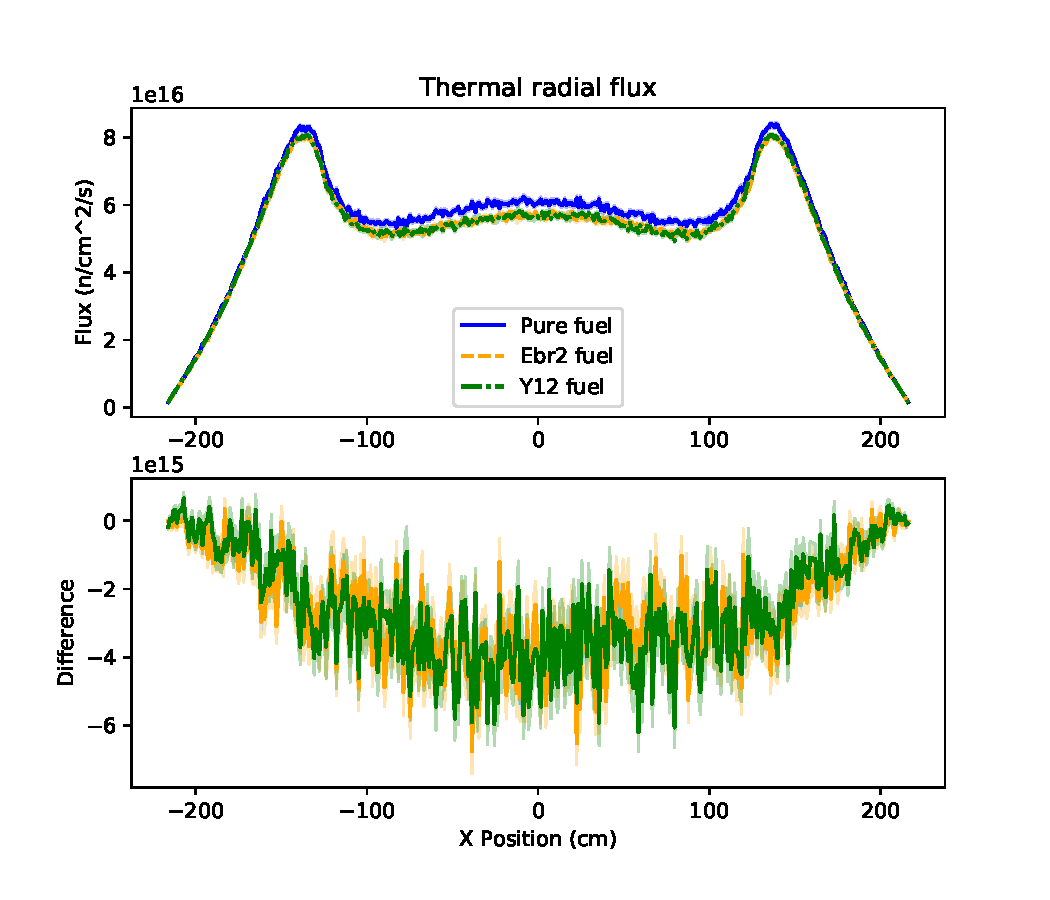
\includegraphics[scale=0.8]{xe100_thermal_radial.pdf}
        \caption{Thermal flux in the Xe-100-like Sangamon200 
        reactor model in the radial direction, across the 
        x-axis.}
        \label{fig:xe100_thermal_radial}
\end{figure}

$^{238}$U has the largest difference between the total and total 
fission cross sections of the uranium isotopes considered for this model. 
So by replacing the U-238 with other isotopes the flux should 
increase from the larger fission to total ratio because the other isotopes 
are more likely to have fission reactions and produce neutrons. But 
another factor to consider is that this core is not just fresh fuel. 
The use of burned pebbles in this model affects the flux because the 
fission yield curves are different for each fissile isotope. 
Also, the even isotopes have relatively small fission cross sections, 
so they're still more likely to absorb a neutron than to fission. 




The fast radial flux (Figure \ref{fig:xe100_fast_radial}) does not 
exhibit the same increases in the reflector as the thermal flux 
because of the neutron energy difference. The fast flux is slightly 
larger than the thermal flux, indicating that more of the neutrons 
in the core are at higher energies. The impure fuels also result in a 
slightly smaller flux in the middle of the core, compared with the  
flux from the pure fuel. The difference in the fluxes is a similar 
order of magnitude to the differences in the thermal fluxes (about 
2-4 $\times 10^{15}$ n/cm$^2$/s), but the fast fluxes are larger than 
the thermal fluxes. Therefore, the impurities result in a smaller 
relative difference in the fast flux than they do in the thermal 
flux. 

\begin{figure}[ht]
        \centering 
        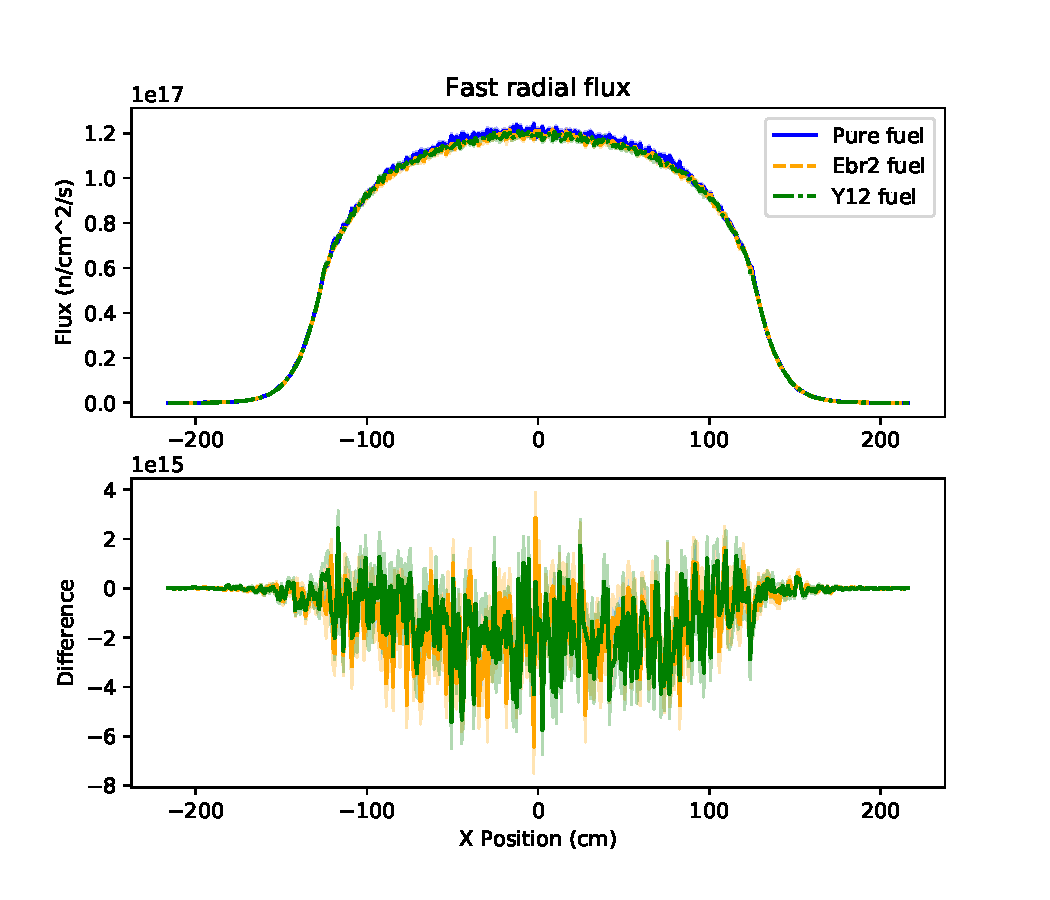
\includegraphics[scale=0.8]{xe100_fast_radial.pdf}
        \caption{Fast flux in the Xe-100-like Sangamon200 
        reactor model in the radial direction, across the 
        x-axis.}
        \label{fig:xe100_fast_radial}
\end{figure}


The thermal axial flux (Figure \ref{fig:xe100_thermal_axial}) shows 
similar results to the thermal radial flux. There is a small bump in the 
flux at the top and bottom of the core because of the graphite reflector.
Additionally, the pure fuel results in a slightly higher flux than 
the impure fuels. The 
two impure fuel compositions result in very similar fluxes. The flux 
differences between the fuel compositions is larger in the bottom 
of the core. The pebble configurations are evenly spaced across the 
core, so the reason for the axial asymmetry in the difference is 
unclear. 

\begin{figure}[ht]
        \centering 
        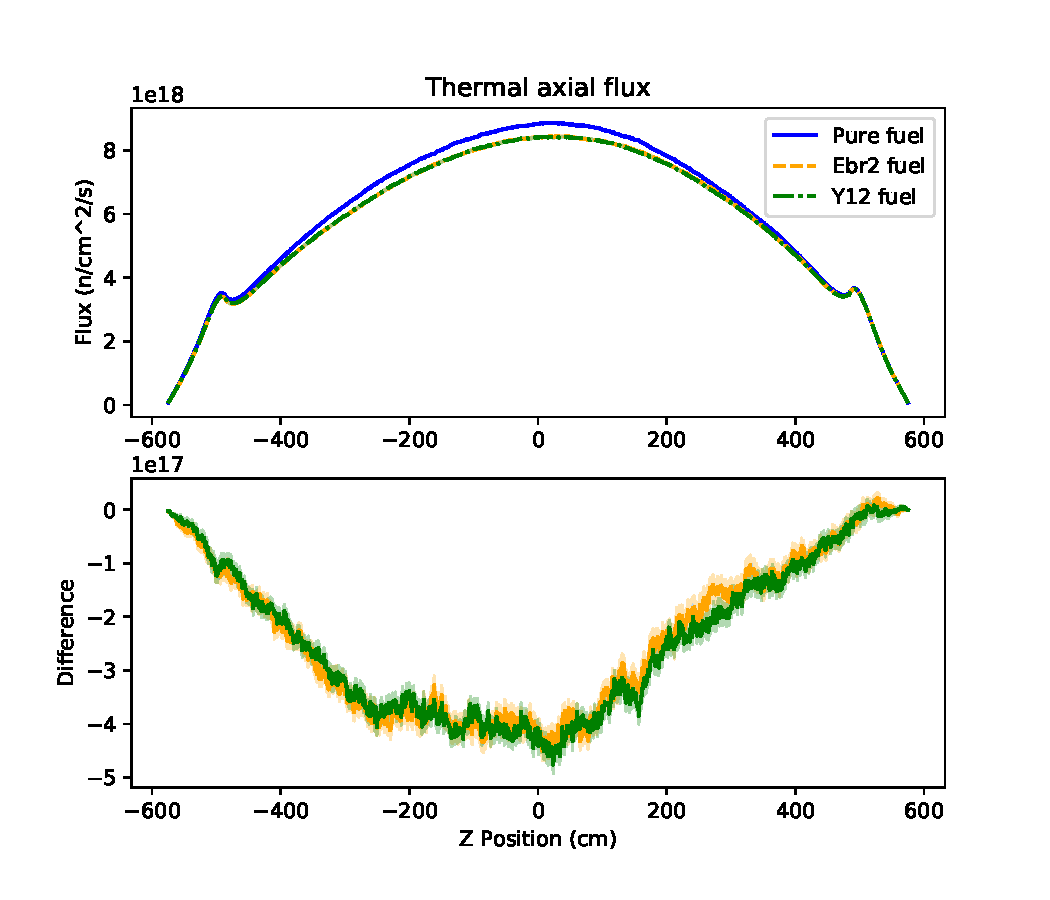
\includegraphics[scale=0.8]{xe100_thermal_axial.pdf}
        \caption{Thermal flux in the Xe-100-like Sangamon200 
        reactor model in the axial direction.}
        \label{fig:xe100_thermal_axial}
\end{figure}

The pure fuel resulting in a larger thermal flux (radially and 
axially) than the impure fuel is consistent with the larger \betaEff 
from this fuel. Delayed neutrons are born in the thermal energy range, 
so a larger \betaEff means that a larger fraction of the neutrons are 
born in the thermal energy range. The difference in \betaEff also explains 
why the relative differences between the fast fluxes from each fuel are 
smaller than the relative differences in the thermal flux: the differences 
in the thermal fluxes are a result of the differences in the fissile 
isotopes present and the delayed neutron precursor groups from each 
fissile isotope. 

The fast axial flux (Figure \ref{fig:xe100_fast_axial}) shows a smaller 
difference in the flux between the different fuel compositions than the 
thermal axial fluxes. The 
impure fuels result in similar fluxes, consistent to observations in 
the thermal axial flux. The largest flux difference between the pure 
and impure fuels is also in the bottom of the core. However, unlike 
in the thermal axial flux, impure fuels result in a slightly larger 
flux than the pure fuel int he top of the core. The axial asymmetry in 
the difference between the fluxes is consistent with the differences in 
the thermal axial fluxes. 

\begin{figure}[ht]
        \centering 
        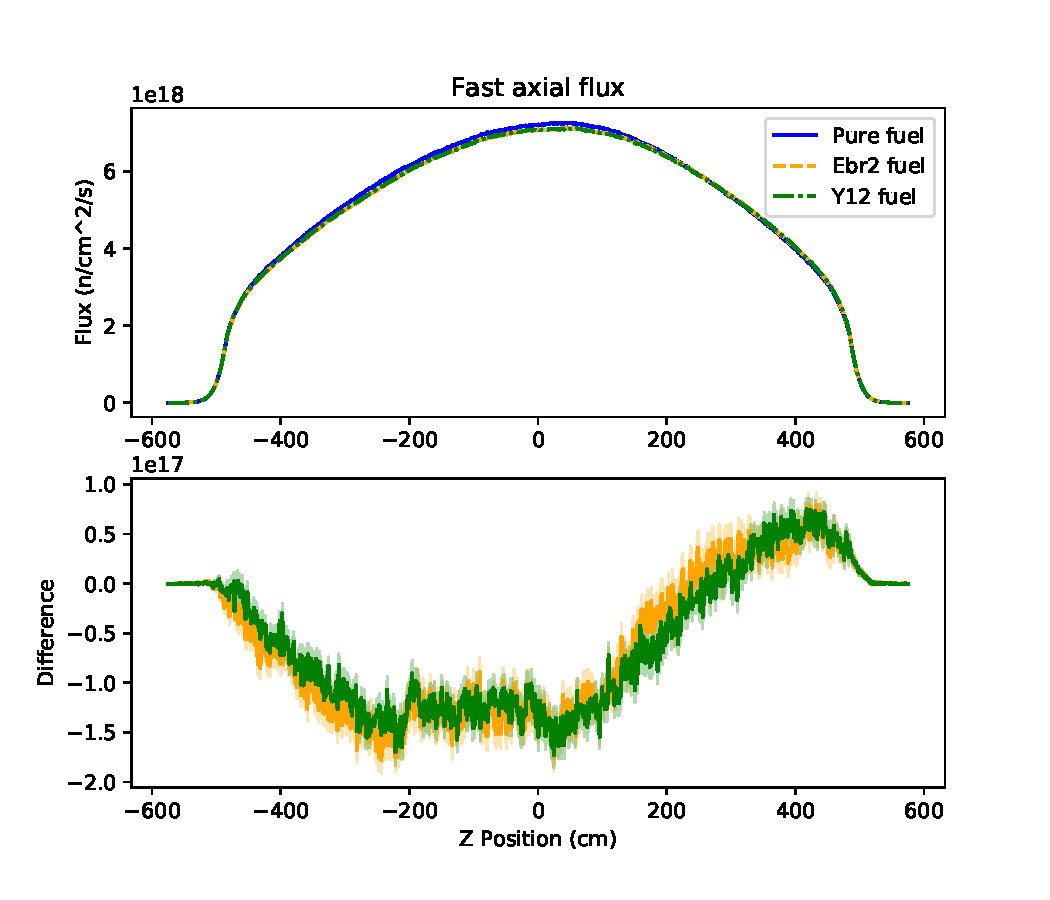
\includegraphics[scale=0.8]{xe100_fast_axial.pdf}
        \caption{Fast flux in the Xe-100-like Sangamon200 
        reactor model in the axial direction.}
        \label{fig:xe100_fast_axial}
\end{figure}

The fluxes from this reactor model are about three orders of 
magnitudes larger than the results from the work by Mulder and 
Boyes \cite{mulder_neutronics_2020}. Part of this difference comes 
from the ranges used for each energy group. Mulder and Boyes used 
a definition of greater than 0.1 MeV and less than 1.86 eV for the 
fast and thermal energy groups, respectively. This work applies a 
definition of greater than 0.625 eV and less then 0.625 eV for fast 
and thermal neutrons, respectively. Therefore, the definitions used by 
Mulder and Boyes does not include all possible neutron energies 
while the definition used in this work does which causes some of the 
differences between the fluxes. 
The other difference leading to the different fluxes comes from the detector 
definitions in the inputs. For this work, the radial detector 
was defined across the x- and y-axes and the axial detector was defined 
across the z-direction. The flux in a detector in Serpent is integrated 
across the volume of the core \cite{leppanen_serpent_2013}. Therefore, 
the flux across any axes not included in the mesh for a detector is 
summed across those axes. This is the primary reason why the flux is 
orders of magnitude different between the two models. 

\subsubsection{Reactivity feedback coefficients}
Table \ref{tab:coeff_xe100} reports the reactivity feedback 
coefficients for each material type in the Xe-100-like reactor model. 
All of the coefficients are negative, which is what is preferred in 
a reactor so that reactivity naturally decreases as temperature increases. 

\begin{table}[ht]
        \centering
        \caption{Reactivity temperature feedback coefficients for 
        each material type in the Xe-100-like model for each fuel 
        type.}
        \label{tab:coeff_xe100}
        \begin{tabular}{c c c c c}
            \hline 
            & \multicolumn{4}{c}{Material feedback coefficinet (pcm/K)} \\
            Fuel Type & Fuel & Coolant & Moderator & Total \\
            \hline
            Pure & -3.875 $\pm$ 0.094 & -0.044 $\pm$ 0.112 & -0.071 $\pm$ 0.459 & -4.216 $\pm$ 0.502\\
            \gls{EBR} & -3.759 $\pm$ 0.138 & -0.433 $\pm$ 0.048 & -0.708 $\pm$ 0.404 & -4.817 $\pm$ 0.438\\
            Y-12 & -3.797 $\pm$ 0.157 & -0.351 $\pm$ 0.092 & -0.728 $\pm$ 0.469 & -4.700 $\pm$ 0.349\\
            \hline

        \end{tabular}
\end{table}

The fuel reactivity feedback coefficient from the pure fuel is more 
negative than the values from the impure fuels, with the \gls{EBR} fuel resulting 
in the least negative fuel feedback coefficient. However, all of 
the values are negative, and are within error of each other. Therefore, 
the fuel composition does not significantly affect this metric. 

For the other three reactivity feedback coefficients, the impure fuels 
result in coefficients that are more negative than the values from 
the pure fuel. The coolant feedback coefficient values are outside 
of the reported error (pure compared with a non-pure fuel), but the 
values of the other two material coefficients are all within error of 
each other. The significant impact on the coolant reactivity feedback 
coefficient suggests that the impurities in the fuel cause a larger 
flux near the single resonance in the total cross section for helium,
resulting in the greater impact from changing this material temperature. 
However based on the values of each material feedback coefficient, 
the coolant temperature has a much smaller effect and impact on the 
total feedback coefficient than the other materials. Therefore even 
though the differences in the coolant feedback coefficient are significant,
they do not have a large impact on the overall operation of the reactor. 


The work by Mulder and Boyes \cite{mulder_neutronics_2020}, reports 
the Doppler coefficient (the fuel feedback), the moderator coefficient, 
and the total coefficient as between -5.6e-5 -- -3.2e-5 $\Delta$ 
\keff/\textdegree C
-4.2e-5 -- -0.4e-4 $\Delta$ \keff/\textdegree C, and -6.1e-5 -- -2e-5 
$\Delta$ \keff/\textdegree C, respectively, for temperatures between 100-900
\textdegree C. The feedback coefficients are within the ranges reported 
by Mulder and Boyes, despite the differences in the reactor models used.
The consistency between the feedback coefficient values from the impure 
fuels in this work and the values reported by Mulder and Boyes suggests that 
the impurities in the fuel do not greatly impact this reactor operation 
metric.  

\subsection{MMR reactor}
The following four sections report and analyze the results of the 
\gls{EBR} and Y-12 impurities in the \gls{MMR}-like reactor model 
created. The four different results are presented for three different 
burnup steps during the reactor operation: \gls{BOL} (0 MWd/kgU),
mid-cycle (40.52 MWd/kgU), and \gls{EOL} (81.04 MWd/kgU). 

\subsubsection{\keff}

Table \ref{tab:mmr_keff} reports the \keff value of the \gls{MMR} at the 
different burnup steps using each fuel composition. At each burnup step, 
using the impure fuel compositions results in a \keff 712-1344 pcm 
smaller than the \keff when using the pure fuel. The difference in \keff 
from the different fuel compositions decreases with burnup because of 
the depletion of the uranium. The impure fuel resulting in a lower \keff 
than the pure fuel is the opposite 
effect of that observed in the Xe-100-like model. The change in the trend 
is because in this reactor the fuel is more homogeneous than in 
the Xe-100-like model. In the Xe-100-like model, the pebbles are modeled 
at different burnup stages, while in this model all of the fuel is at the 
same burnup step. All of the fuel in this model is unburned in the 
first burnup step, meaning that the impurities have a more significant 
effect on the neutron population because the impurities are a larger fraction 
of the uranium in the core than in the Xe-100-like model.

\begin{table}[ht]
        \centering
        \caption{\keff in the \gls{MMR}-like model at select burnup 
        steps.}
        \label{tab:mmr_keff}
        \begin{tabular}{c c c c}
                \hline 
                & \multicolumn{3}{c}{Burnup step}\\
                Fuel Type & \gls{BOL} & Mid-cycle & \gls{EOL} \\
                \hline 
                Pure & 1.33797 $\pm$ 0.00027 & 1.18048 $\pm$ 0.00025 & 1.05535$\pm$000024\\
                \gls{EBR} & 1.32609 $\pm$0.00028 & 1.17148 $\pm$ 0.00027 & 1.04792 $\pm$ 0.00025 \\
                Y-12 & 1.32453$\pm$0.00029 & 1.17051$\pm$0.00027 & 1.04823$\pm$0.0024\\
                \hline
                
        \end{tabular}
\end{table}

 

The effect of of the impurities on this reactor model are significant on the 
\keff because the differences are more than the error on the values. However, 
even at the last burnup step, which is at the end of life for the reactor 
core, the \keff is still above 1. Therefore the effect of the impurities 
is not great enough to cause the reactor to reach a subcritical state 
during its operation. The super-critical \keff throughout the duration 
of the burn cycle suggests that the lifetime of the reactor will not be 
affected by the impurities in the fuel.

\subsubsection{\betaEff}

Table \ref{tab:mmr_betaeff} reports the \betaEff values when using 
each fuel composition at the different burnup steps. For all three 
fuel compositions, the \betaEff decreases with increasing burnup. This 
is consistent with the depletion of the $^{235}$U in the core and 
an increase in the number of fissions happening in isotopes
that have a lower \betaEff than $^{235}$U, such as $^{239}$Pu. 
Additionally, the \betaEff values at \gls{BOL} are slightly larger 
than the expected 0.0064 value of $\beta$ for thermal fissions in $^{235}$U
or the \betaEff of a typical \gls{PWR}. This effect is because the 
small size of the core and higher enrichment causing the 
increase in the probability of non-leakage of fast neutrons to 
dominate the decrease of the fast fission factor. 

\begin{table}[ht]
        \centering
        \caption{\betaEff value in the \gls{MMR}-like model at 
        select burnup steps.}
        \label{tab:mmr_betaeff}
        \begin{tabular}{c c c c}
                \hline 
                 & \multicolumn{3}{c}{Burnup step}\\
                Fuel & \gls{BOL} & Mid-cycle & \gls{EOL}\\
                \hline 
                Pure & 0.00669 $\pm$ 0.00004 & 0.00586 $\pm$ 0.00004 & 0.00548 $\pm$ 0.00003\\
                \gls{EBR} & 0.00663 $\pm$ 0.00003 & 0.00591 $\pm$ 0.00003 & 0.00542 $\pm$ 0.00003\\
                Y-12 & 0.00665 $\pm$ 0.00004 &  0.00598 $\pm$ 0.00004& 0.00553 $\pm$ 0.00003\\
                \hline 

        \end{tabular}
\end{table}

Each of the fuel compositions result in different \betaEff values at 
each burnup step. However, almost all of the values from the impure 
fuels are within error of the value from the pure fuel. Therefore, the 
fuel impurities do not lead to any significant changes in the 
\betaEff. Additionally, the impure fuel compositions do not lead to 
a consistent change in \betaEff between burnup steps. 

\subsubsection{Neutron Flux}

Figure \ref{fig:mmr_energy_spectrum} shows the flux in the active 
region of the core as a function of energy (top) and the difference between 
the flux from the pure fuel and each of the impure fuels (bottom). This 
data was 
calculated using the defined SCALE-238 energy group structure in Serpent,
with the plotted flux of each group normalized by lethargy. The purple 
line in both plots in the figure shows the delineation between the fast and 
thermal energy groups. This figure shows that the difference between 
the fluxes is small compared with the magnitude of the flux, especially in 
the thermal group (left of the purple line). The difference between the 
fluxes generally increases with energy such that the largest difference in 
in the peak around 1 MeV. However, this difference is about two orders 
of magnitude smaller than the flux. The differences 
in the flux from the pure fuel and the flux from each of the impure 
fuels is larger in the fast energy group than in the thermal energy group.

\begin{figure}
        \centering
        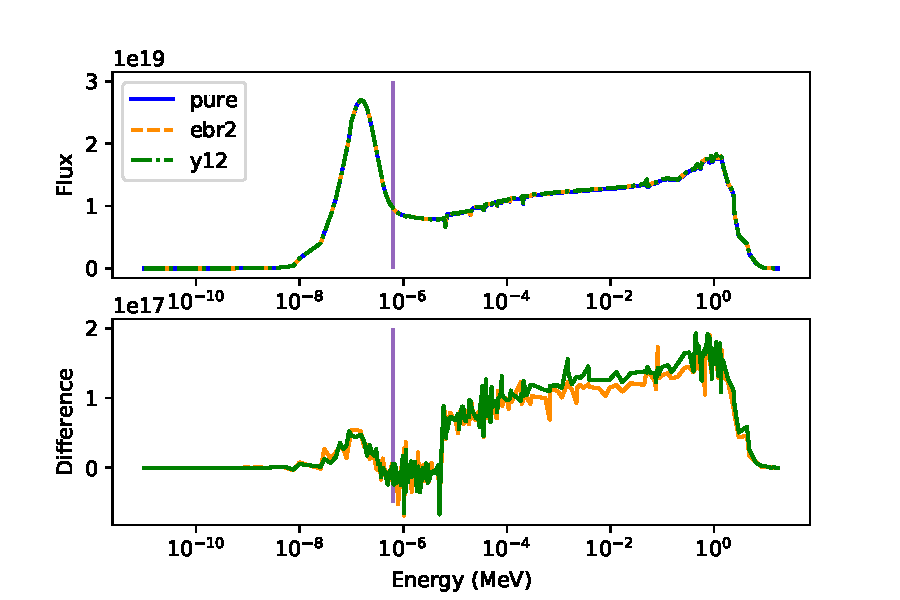
\includegraphics{mmr_energy_spectrum.pdf}
        \caption{Top: Flux energy spectrum for each fuel composition at a 
        burnup of 0 MWd/kgU in the active region of the core. The 
        purple line shows the delineation between the fast and thermal 
        neutron energy groups used in other results of this work. \\
        Bottom: Difference between the flux from the pure fuel and each 
        of the impure fuels in each energy group. The purple line shows the 
        delineation between the fast and thermal energy groups. }
        \label{fig:mmr_energy_spectrum}
\end{figure}

Figures \ref{fig:mmr_bol}-\ref{fig:mmr_eol} show the neutron flux 
in the thermal and fast energy ranges in the radial and axial 
direction for each burnup step. The radial fluxes are taken 
across the middle of the core in the y-direction, which means the flux 
is taken across the plane with three coolant channels in Figure 
\ref{fig:mmr_radial}. The axial flux is taken along the z-axis, with the 
x- and y-directions collapsed. 

The radial flux at \gls{BOL} (Figures \ref{fig:mmr_thermal_radial_bol} and 
\ref{fig:mmr_fast_radial_bol}) show that the thermal flux peaks in the 
control rod channels and the fast flux has a trough in these regions. 
Conversely, the thermal flux has a trough in the areas closest to the fuel 
channels and the fast flux has a peak in these areas.
The greatest difference in the 
fluxes between the fuel compositions is in the areas of the core close 
to the fuel pellets, where the thermal flux troughs and the fast flux 
peaks. This result is consistent with only the fuel 
composition changing between each core model, as the different fuel 
compositions would lead to different energy spectrums for the neutrons 
born form fission and thermalizing in the graphite around the fuel channels.
The fast flux along tis axis is larger than the thermal flux, which is 
consistent with the observation of the active-core flux as a function of 
energy. Unlike in the Xe-100-like core model, the impure fuels do not 
result in a consistent difference from the flux of the pure fuel; the 
differences in the fluxes are more of a function of the location 
in the core than the fuel type.

\begin{figure}[ht]
        \centering
        \begin{subfigure}[b]{0.48\textwidth}
            \centering
            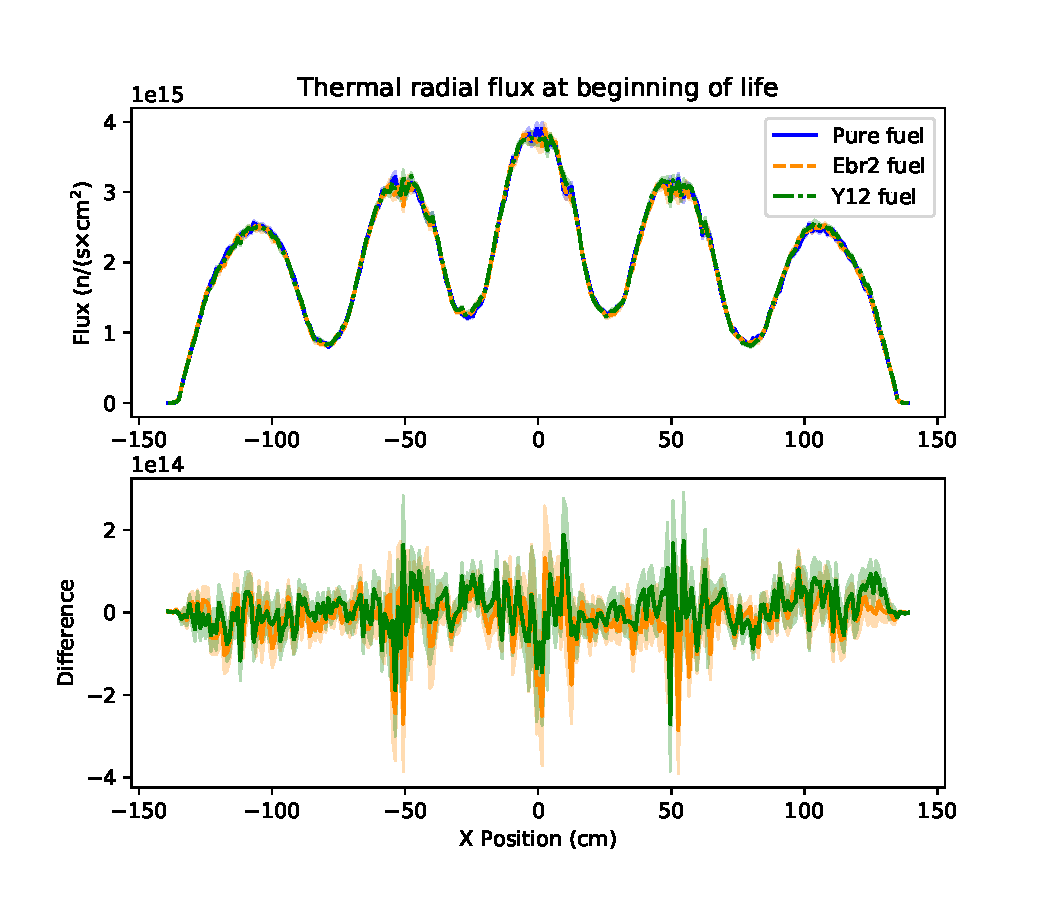
\includegraphics[width=\textwidth]{mmr_thermal_radial_bol.pdf}
            \caption{Thermal radial flux in the \gls{MMR}-like reactor.}
            \label{fig:mmr_thermal_radial_bol}
        \end{subfigure}
        \hfill
        \begin{subfigure}[b]{0.48\textwidth}
            \centering
            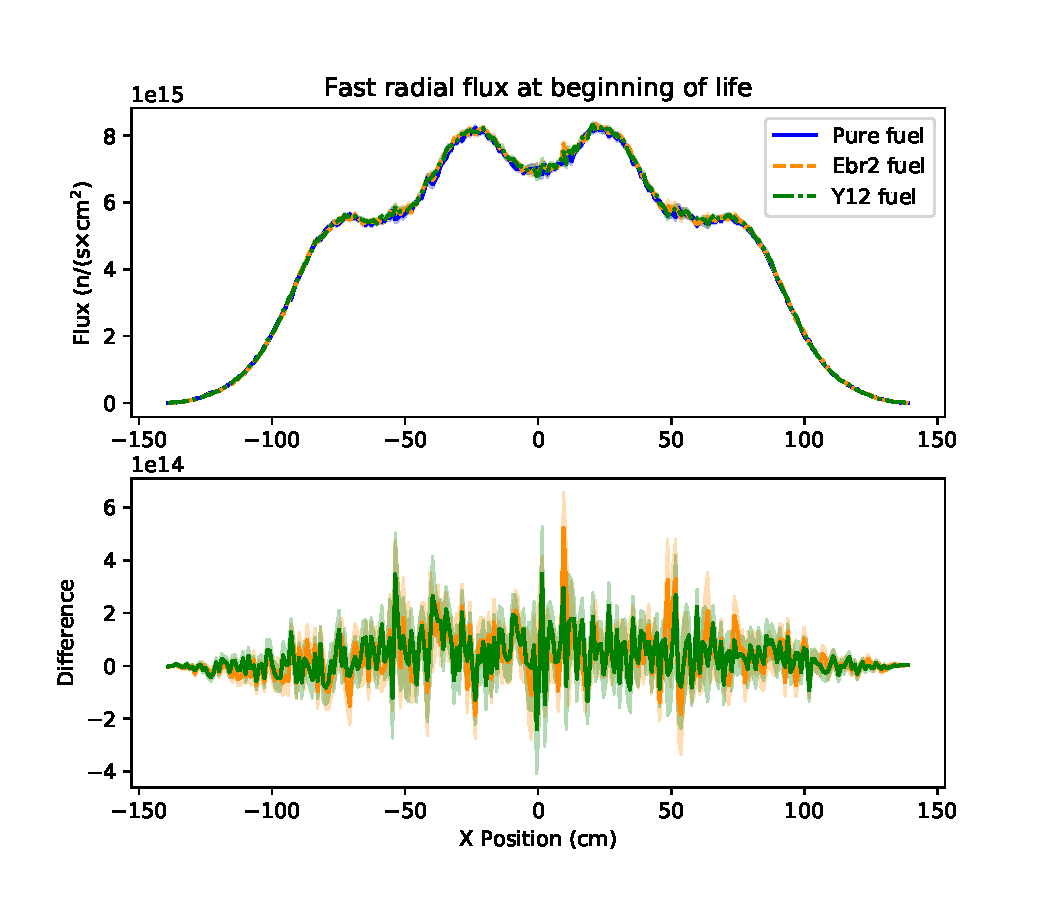
\includegraphics[width=\textwidth]{mmr_fast_radial_bol.pdf}
            \caption{Fast radial flux in the \gls{MMR}-like reactor.}
            \label{fig:mmr_fast_radial_bol}
        \end{subfigure}
        \hfill            
        \begin{subfigure}[b]{0.48\textwidth}
            \centering
            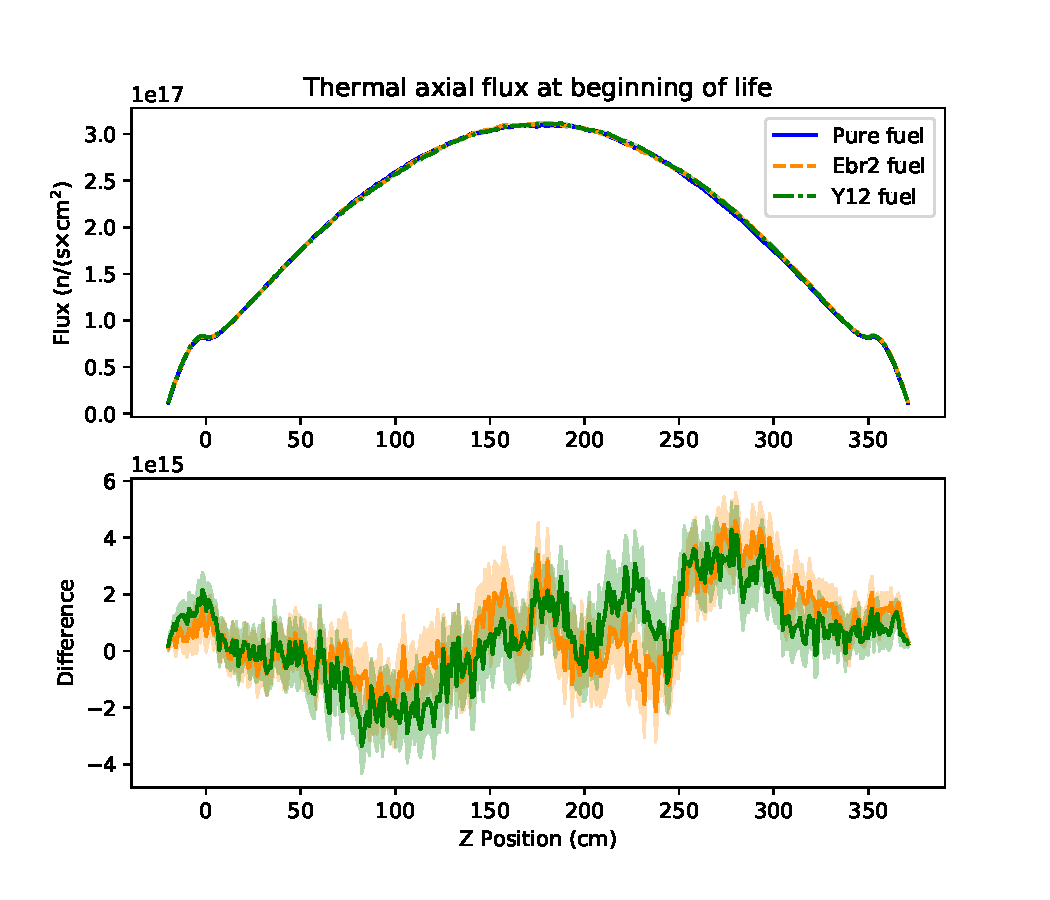
\includegraphics[width=\textwidth]{mmr_thermal_axial_bol.pdf}
            \caption{Thermal axial flux in the \gls{MMR}-like reactor. }
            \label{fig:mmr_thermal_axial_bol}
        \end{subfigure}
        \hfill
        \begin{subfigure}[b]{0.48\textwidth}
            \centering
            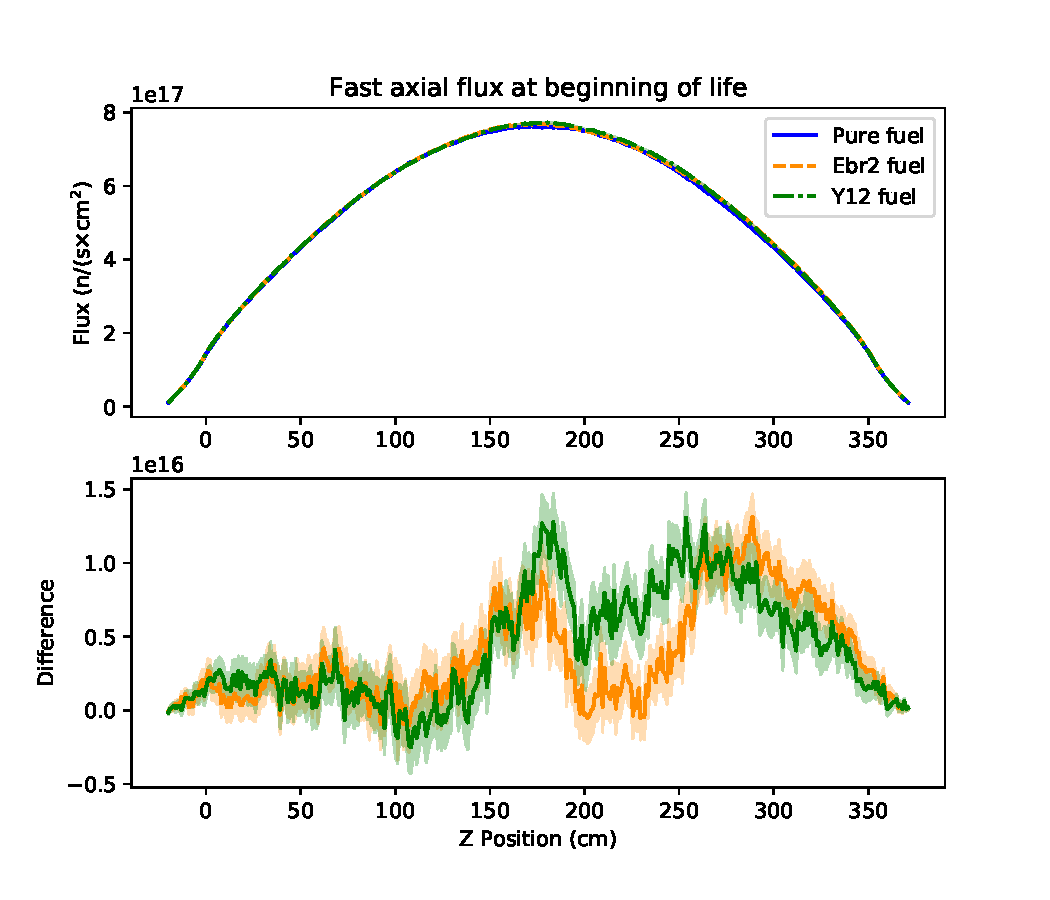
\includegraphics[width=\textwidth]{mmr_fast_axial_bol.pdf}
            \caption{Fast axial flux in the \gls{MMR}-like reactor.}
            \label{fig:mmr_fast_axial_bol}
        \end{subfigure}
        \hfill
        \caption{Radial and axial flux for each energy group when using 
        each fuel composition in the \gls{MMR}-like model at the beginning 
        of life.}
        \label{fig:mmr_bol}
   \end{figure}

The axial fluxes at \gls{BOL} (Figures \ref{fig:mmr_thermal_axial_bol} and 
\ref{fig:mmr_fast_axial_bol}) show the effect of the graphite moderators at 
the top and bottom of the core. The thermal flux has a small peak in the 
moderator wile the fast flux has a small exponential decrease in the 
moderator. The fluxes also show that using the impure fuels results in 
a slightly smaller flux at the bottom of the core and a slightly higher 
flux at the top of the core. This axial asymmetry is consistent with 
the results of the Xe-100-like core model. The differences between the 
fluxes is 1-2 orders of magnitude smaller than the flux, but is 
still one order of magnitude larger than the error of the fluxes.

Figure \ref{fig:mmr_mc} shows the different fluxes in the \gls{MMR}-like 
reactor at mid-cycle. The trends at mic-cycle in the radial fluxes are 
similar to those observed at the \gls{BOL}: the radial fluxes have the 
greatest difference near the fuel pins in the core. In the axial fluxes 
however, there is a noticeable difference between the flux from the \gls{EBR} 
fuel and the other fuels. The \gls{EBR} results in a greater difference 
from the flux from the pure fuel than the Y-12 fuel, but the shape of 
the difference is similar to what was observed at \gls{BOL}; the flux from 
the \gls{EBR} fuel is less than that from the pure fuel in the bottom of 
the core and greater at the top of the core. For the thermal axial flux, 
the difference between the flux from the pure and Y-12 fuels decreases 
compared with the fluxes at \gls{BOL}, but the difference between the flux 
from pure and \gls{EBR} fuel increases compared with the flux at \gls{BOL}. 
A similar pattern occurs in the fast axial flux. This suggests that 
as the core burns, the impurities in the Y-12 fuel are burned off sooner 
than those present in the \gls{EBR} or that the impurities breed material 
similar to what is present in the pure fuel as it burns. 

\begin{figure}
        \centering
        \begin{subfigure}[b]{0.48\textwidth}
            \centering
            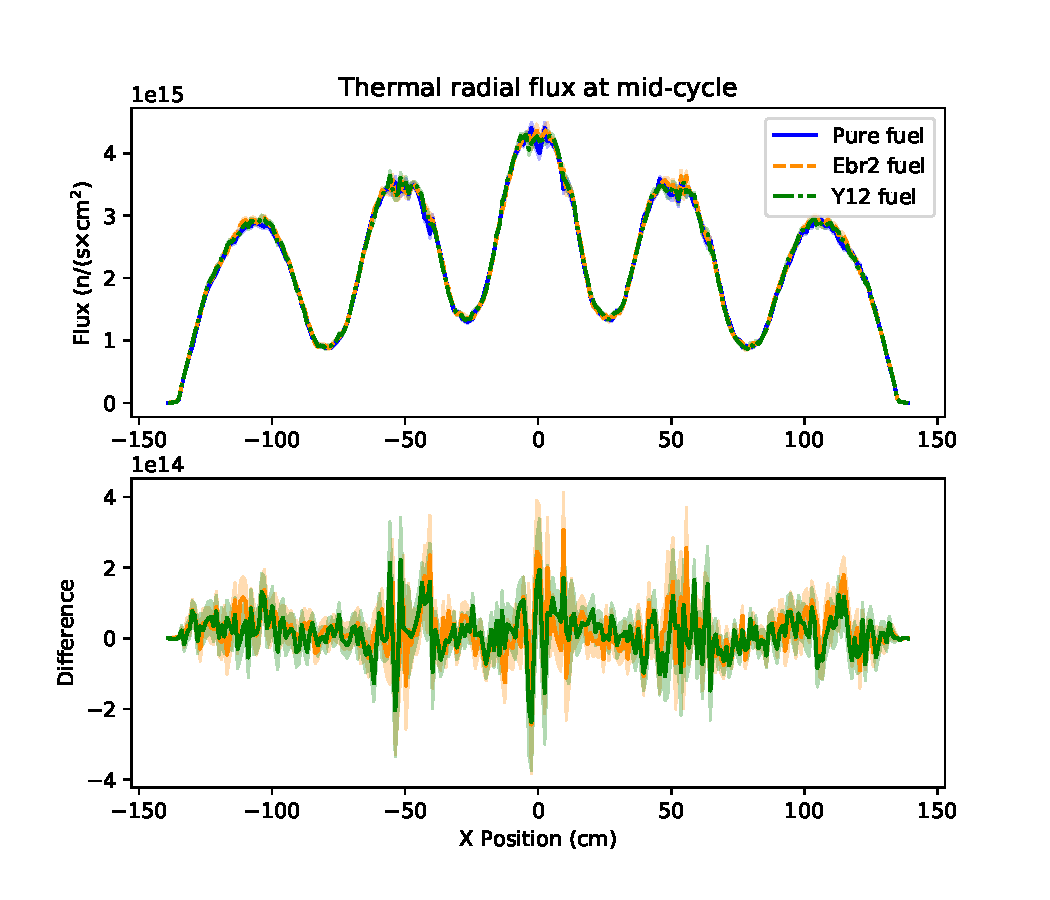
\includegraphics[width=\textwidth]{mmr_thermal_radial_mc.pdf}
            \caption{Thermal radial flux in the \gls{MMR}-like reactor.}
            \label{fig:mmr_thermal_radial_mc}
        \end{subfigure}
        \hfill
        \begin{subfigure}[b]{0.48\textwidth}
            \centering
            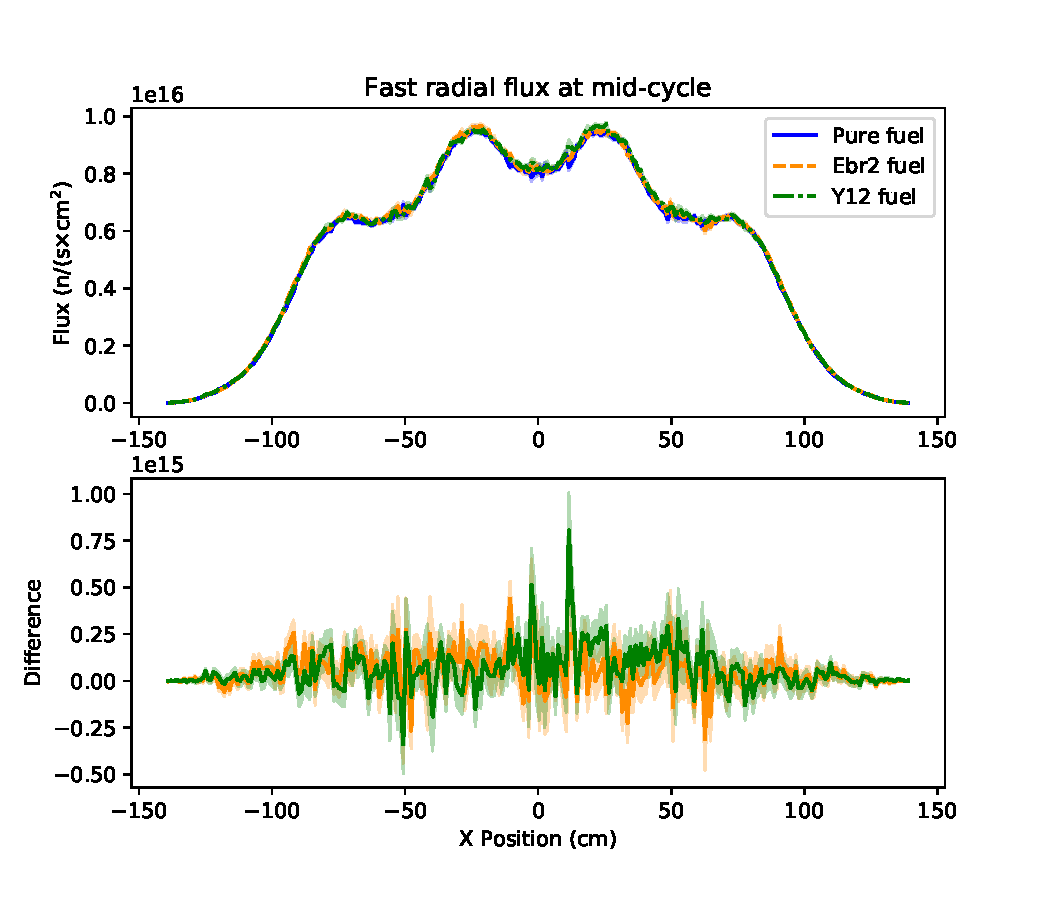
\includegraphics[width=\textwidth]{mmr_fast_radial_mc.pdf}
            \caption{Fast radial flux in the \gls{MMR}-like reactor.}
            \label{fig:mmr_fast_radial_mc}
        \end{subfigure}
        \hfill
            
        \begin{subfigure}[b]{0.48\textwidth}
            \centering
            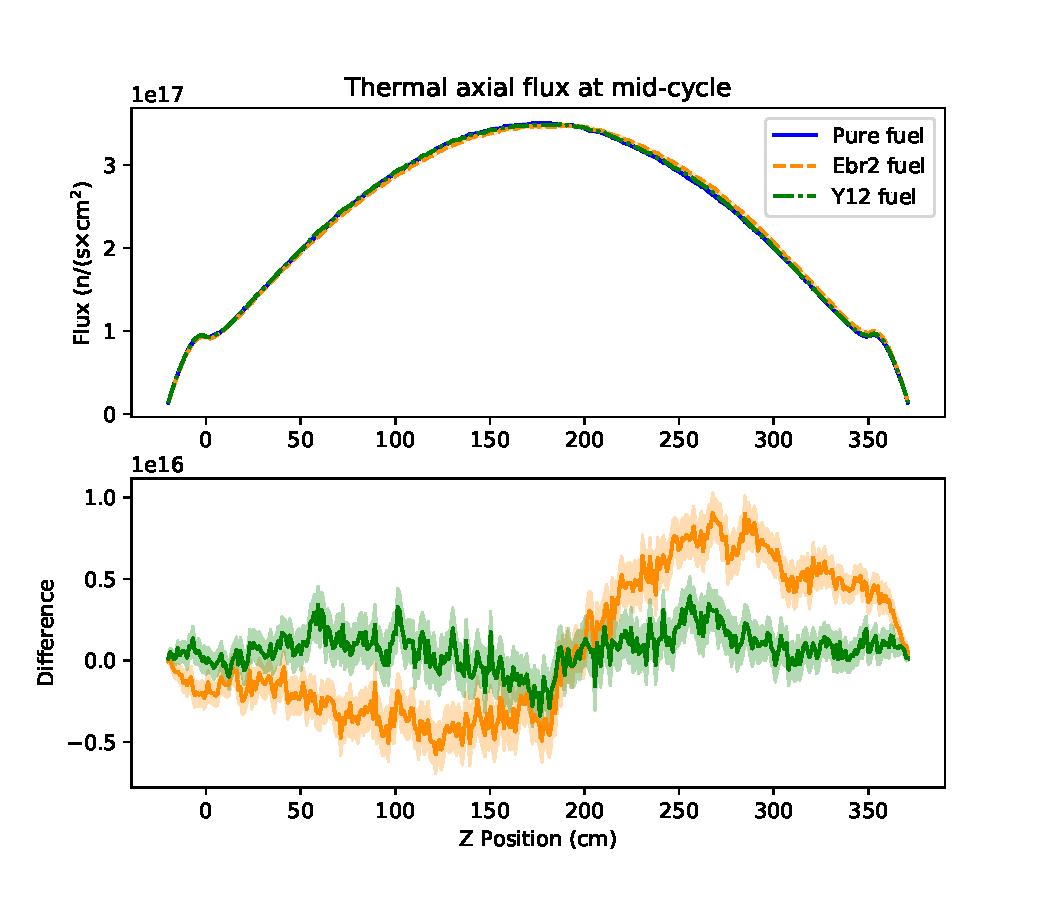
\includegraphics[width=\textwidth]{mmr_thermal_axial_mc.pdf}
            \caption{Thermal axial flux in the \gls{MMR}-like reactor. }
            \label{fig:mmr_thermal_axial_mc}
        \end{subfigure}
        \hfill
        \begin{subfigure}[b]{0.48\textwidth}
            \centering
            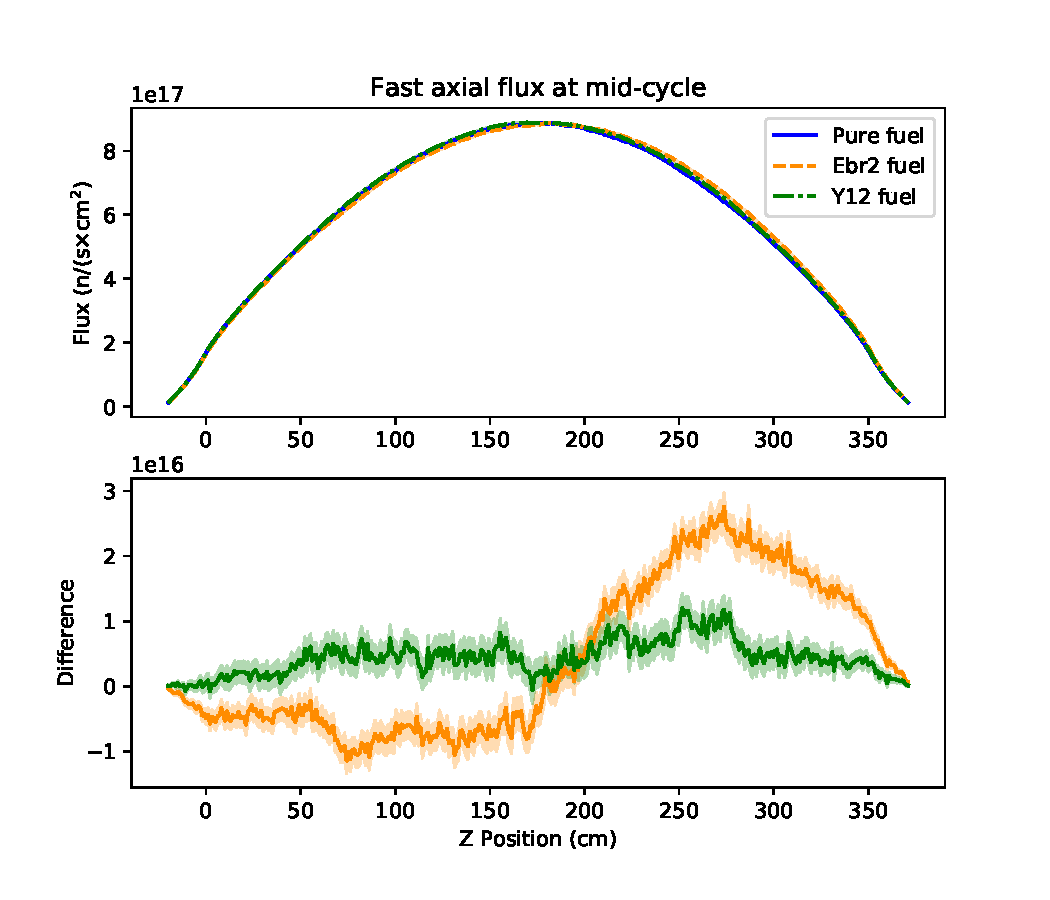
\includegraphics[width=\textwidth]{mmr_fast_axial_mc.pdf}
            \caption{Fast axial flux in the \gls{MMR}-like reactor.}
            \label{fig:mmr_fast_axial_mc}
        \end{subfigure}
        \hfill
        \caption{Radial and axial flux for each energy group when using 
        each fuel composition in the \gls{MMR}-like model at middle of 
        the operation cycle.}
        \label{fig:mmr_mc}
   \end{figure}

Finally, Figure \ref{fig:mmr_eol} shows the different fluxes in the 
\gls{MMR}-like model at \gls{EOL}. The radial fluxes continue to show 
the same trend of the largest differences between the fluxes occurring near
the fuel pins. The axial fluxes (Figures \ref{fig:mmr_thermal_axial_eol} and 
\ref{fig:mmr_fast_axial_eol}) show a different trend. Both axial 
fluxes show that the impure fuels result in a larger flux at the 
bottom of the core and a smaller flux at the top of the core than the flux 
from the pure fuel, opposite
to what was observed in the \gls{BOL} and mid-cycle fluxes. The thermal 
and fast axial fluxes are higher at the \gls{EOL} than at the other 
two burnup steps. The difference between the flux from \gls{EBR} fuel 
and the pure fuel decreases from the difference at mid-cycle, but the 
difference between the fluxes from the pure and Y-12 fuel 
increases from the difference at mid-cycle. 
   
\begin{figure}
        \centering
        \begin{subfigure}[b]{0.48\textwidth}
            \centering
            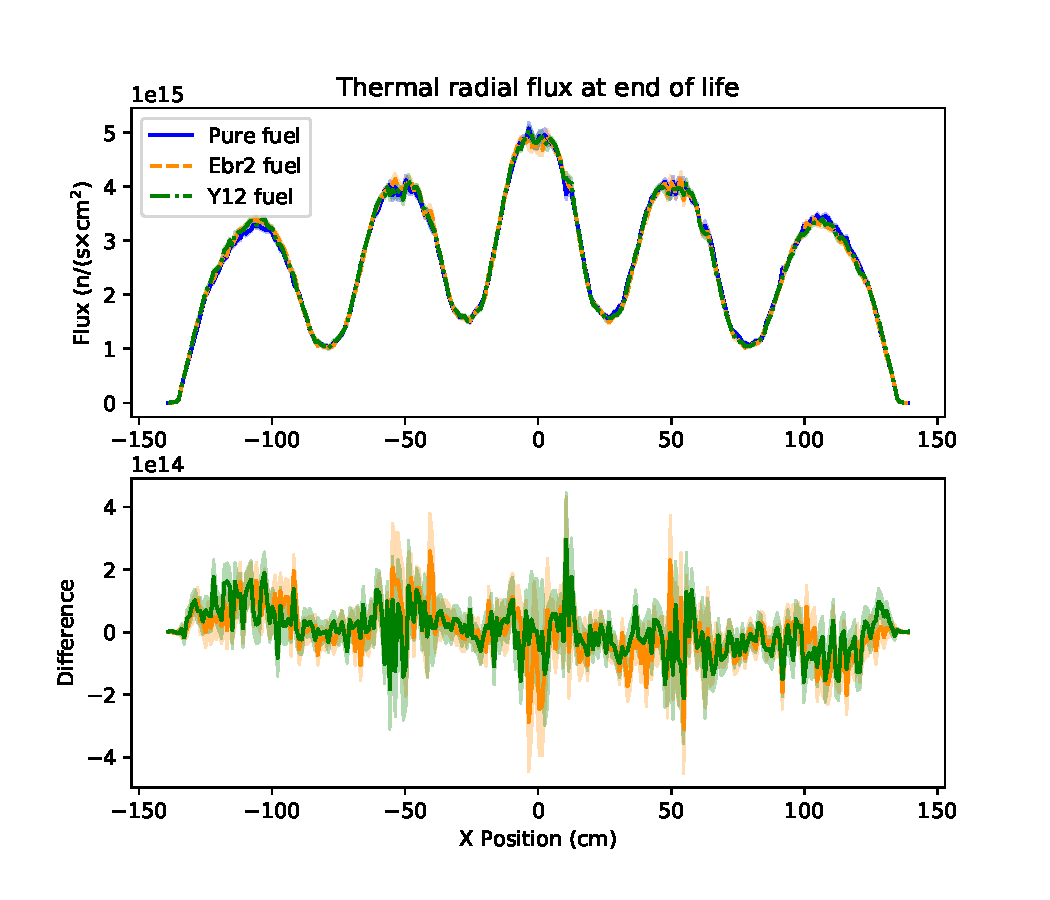
\includegraphics[width=\textwidth]{mmr_thermal_radial_eol.pdf}
            \caption{Thermal radial flux in the \gls{MMR}-like reactor.}
            \label{fig:mmr_thermal_radial_eol}
        \end{subfigure}
        \hfill
        \begin{subfigure}[b]{0.48\textwidth}
            \centering
            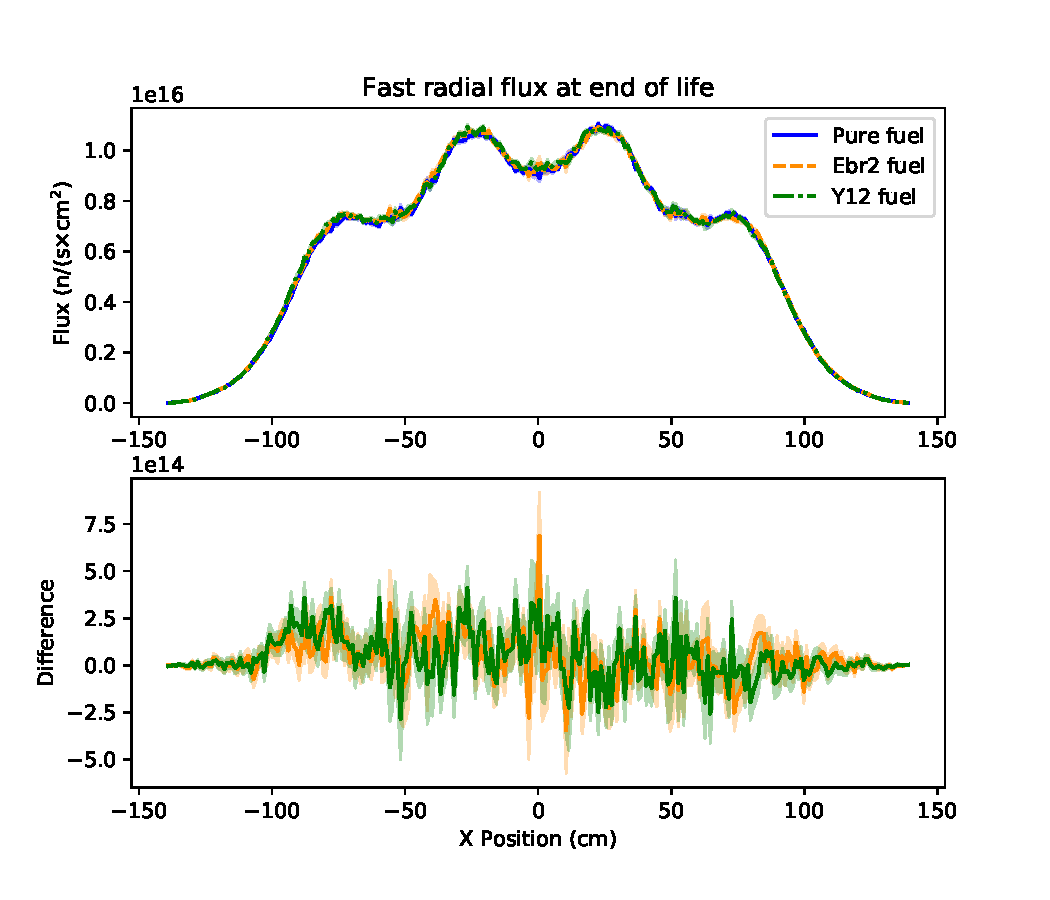
\includegraphics[width=\textwidth]{mmr_fast_radial_eol.pdf}
            \caption{Fast radial flux in the \gls{MMR}-like reactor.}
            \label{fig:mmr_fast_radial_eol}
        \end{subfigure}
        \hfill
            
        \begin{subfigure}[b]{0.48\textwidth}
            \centering
            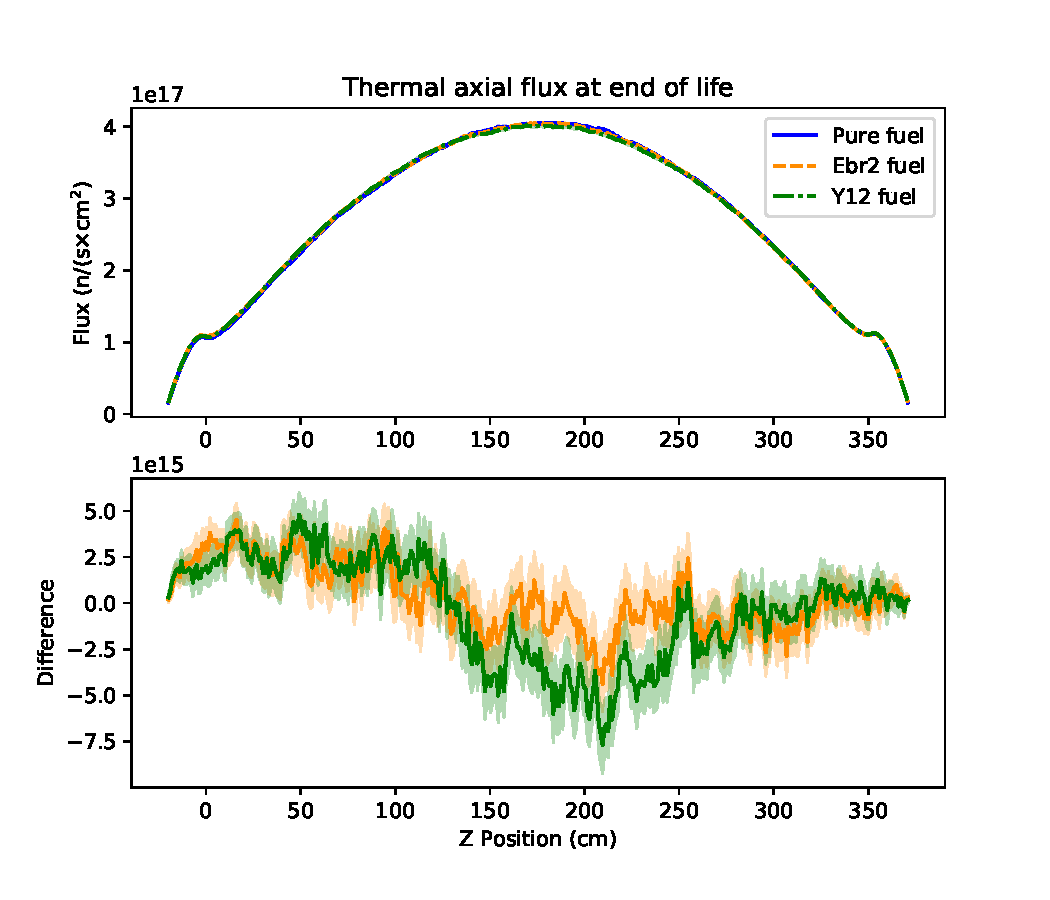
\includegraphics[width=\textwidth]{mmr_thermal_axial_eol.pdf}
            \caption{Thermal axial flux in the \gls{MMR}-like reactor. }
            \label{fig:mmr_thermal_axial_eol}
        \end{subfigure}
        \hfill
        \begin{subfigure}[b]{0.48\textwidth}
            \centering
            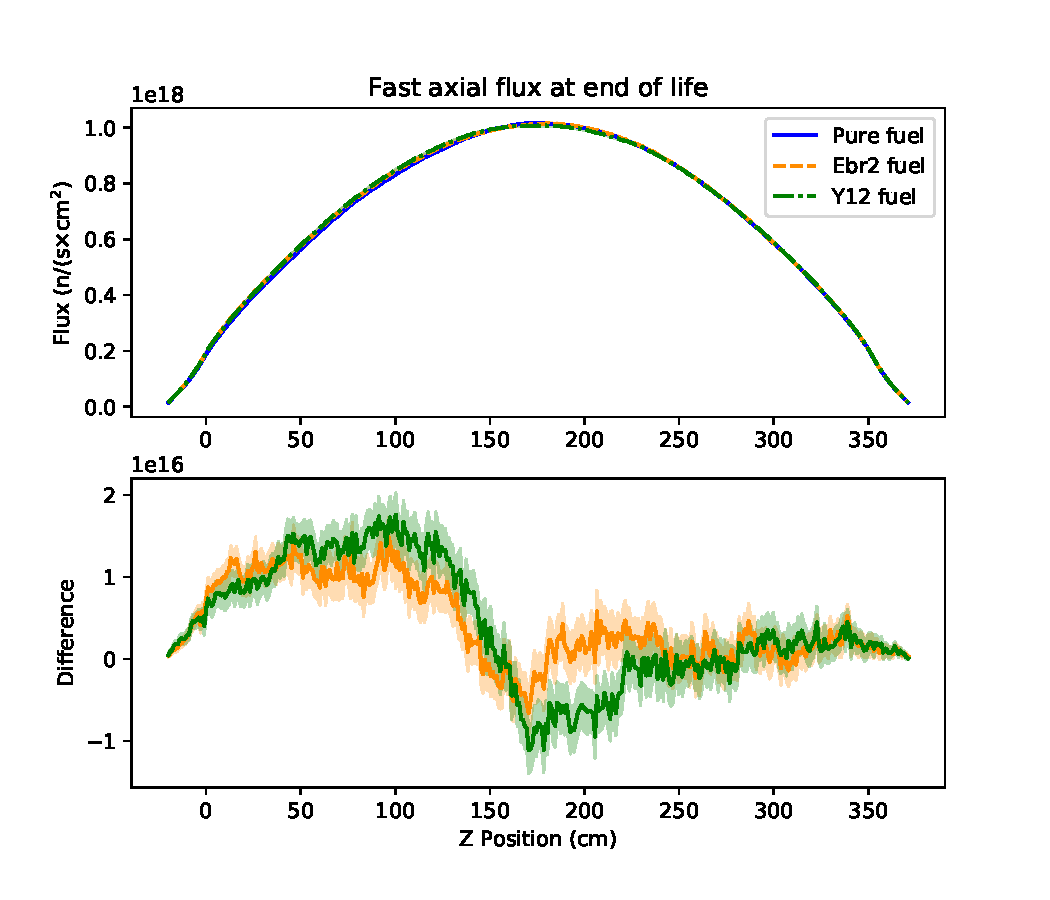
\includegraphics[width=\textwidth]{mmr_fast_axial_eol.pdf}
            \caption{Fast axial flux in the \gls{MMR}-like reactor.}
            \label{fig:mmr_fast_axial_eol}
        \end{subfigure}
        \hfill
        \caption{Radial and axial flux for each energy group when using 
        each fuel composition in the \gls{MMR}-like model at the end 
        of life.}
        \label{fig:mmr_eol}
   \end{figure}


\subsubsection{Reactivity feedback coefficients}
Finally, the reactivity feedback coefficients of different materials 
at each burnup step are reported in Table \ref{tab:coeff_mmr}. The 
fuel reactivity feedback coefficients become more negative with 
burnup, because the $^{235}$U in the core depleted with burnup, 
leaving a larger relative abundance of $^{238}$U and $^{239}$Pu in 
the core, which both have more resonances than $^{235}$U. The 
additional resonances of the $^{238}$U and ${239}$Pu means that the 
Doppler broadening effect has a more pronounced impact on the reactivity 
of the core. At each of the burnup steps, the different fuel compositions 
result in different fuel reactivity coefficients, but each of the values 
are within error of each other. The values being within error suggests 
that the fuel composition does not have a significant effect on 
this parameter. 

\begin{table}
        \centering 
        \caption{Reactivity feedback coefficients (pcm/K) for different 
        materials at different burnup steps in the \gls{MMR}-like 
        reactor model.}
        \label{tab:coeff_mmr}
        \begin{tabular}{c c c c}
                \hline 
                & \multicolumn{3}{c}{Burnup step} \\
                Fuel & \gls{BOL} & Mid-cycle & \gls{EOL} \\
                \hline 
                \multicolumn{4}{c}{Fuel reactivity feedabck}\\
                Pure & -3.314 $\pm$ 0.059 & -3.889 $\pm$ 0.088 & -4.536 $\pm$0.264\\
                \gls{EBR} & -3.073 $\pm$ 0.109 & -3.720 $\pm$ 0.147 & -4.699 $\pm$ 0.151\\
                Y-12 & -3.233 $\pm$ 0.107 & -3.704 $\pm$ 0.133 & -4.168 $\pm$ 0.100\\
                \hline 
                \multicolumn{4}{c}{Coolant reactivity feedabck}\\
                Pure & -0.211 $\pm$ 0.063 & 0.021 $\pm$ 0.169 & 0.052 $\pm$ 0.234\\
                \gls{EBR} & 0.007 $\pm$ 0.051 & -0.165 $\pm$ 0.183 & 0.005 $\pm$ 0.085\\
                Y-12 & -0.221 $\pm$ 0.068 & 0.197 $\pm$ 0.145 & -0.0146 $\pm$ 0.158\\
                \hline 
                \multicolumn{4}{c}{Moderator reactivity feedabck}\\
                Pure & -0.815 $\pm$ 0.062 & -1.298 $\pm$ 0.155 & -2.590 $\pm$ 0.323\\
                \gls{EBR} &-0.934 $\pm$ 0.171 & -1.723 $\pm$ 0.268 & -2.375 $\pm$ 0.313\\
                Y-12 & -0.950 $\pm$ 0.138 & -1.333 $\pm$ 0.206 & -2.432 $\pm$ 0.190\\
                \hline 
                \multicolumn{4}{c}{Total reactivity feedabck}\\
                Pure & -4.142 $\pm$ 0.297 & -5.015 $\pm$ 0.215 & -6.865 $\pm$ 0.300\\
                \gls{EBR} & -4.191 $\pm$ 0.097 & -5.284 $\pm$ 0.286 & -6.709 $\pm$ 0.329\\
                Y-12 & -4.037 $\pm$ 0.322 & -5.410 $\pm$ 0.268 & -6.689 $\pm$ 0.232\\
                \hline 
                
                
        \end{tabular}
\end{table}

The coolant reactivity feedback coefficients have the smallest absolute 
value of any of the coefficients considered in this work, which 
indicates that the helium coolant has the smallest effect on the reactivity 
of the core as the temperature changes. Additionally, the coolant 
reactivity feedback coefficient is not at dependent on the burnup of the 
fuel like the other coefficients. This is a result of the density change 
being the primary temperature-dependent property of the helium coolant, 
instead of widening of cross section resonances. 
At the \gls{BOL}, the \gls{EBR} fuel results in a statistically different 
coolant feedback coefficient, which shows that the fuel composition has some 
impact on this parameter. However, the coolant reactivity feedback 
coefficient is small compared to the other feedback coefficients so this 
change is unlikely to cause significant changes in the operation of the 
core as a whole. 

The moderator feedback coefficient is negative for each of the fuel 
compositions at each burnup step, indicating that this core is 
undermoderated. This feedback coefficient also becomes more 
negative with burnup, because the flux in the core increases with 
burnup. The increase in flux means that the resonance broadening has more 
of an effect on the reactivity of the core. At the \gls{BOL} and 
mid-cycle steps the pure fuel has the least negative moderator 
feedback coefficient, but at \gls{EOL} the pure fuel has the most 
negative coefficient. However, at each of the burnup steps the moderator 
feedback coefficient from each of the fuels are within error of each 
other. This agreement within error suggests that the fuel composition 
does not have a significant effect on this reactor operation parameter. 

Finally, the total reactivity feedback coefficients are also all negative 
for each fuel composition at each burnup step, and they become more 
negative with burnup. Based on the values of the feedback 
coefficients for each individual material, the total feedback coefficient 
is mostly driven by the fuel feedback coefficient at each burnup step. 
The different fuel compositions result in total reactivity feedback 
coefficients that are within error of each other. Therefore, the fuel 
composition does not significantly affect this reactor parameter either. 

At each burnup step, the fuel and total reactivity feedback coefficients are 
negative for each fuel composition and the values from each fuel composition 
are within error of each other. These two results suggests that the fuel 
composition will not prevent this reactor design from operating in a safe 
state. 